
\documentclass[oneside, 11 pt]{report}
\usepackage{hyperref, graphicx}
\title{Internet of thing}
\date{\today}
\author{Rihan Ali Ripon \\ \href{mailto:ripon365cse@gmail.com}{ripon365cse@gmail.com}}
\begin{document}
\maketitle


\section*{Introduction}
The Internet of Things (IoT) is a system of interrelated computing devices, mechanical and digital machines, objects, animals or people that are provided with unique identifiers and the ability to transfer data over a network without requiring human-to-human or human-to-computer interaction.

The definition of the Internet of Things has evolved due to the convergence of multiple technologies, real-time analytics, machine learning, commodity sensors, and embedded systems. Traditional fields of embedded systems, wireless sensor networks, control systems, automation (including home and building automation), and others all contribute to enabling the Internet of Things. In the consumer market, IoT technology is most synonymous with products pertaining to the concept of the "smart home", covering devices and appliances (such as lighting fixtures, thermostats, home security systems and cameras, and other home appliances) that support one or more common ecosystems, and can be controlled via devices associated with that ecosystem, such as smartphones and smart speakers.

There are a number of serious concerns about dangers in the growth of IoT, especially in the areas of privacy and security, and consequently industry and governmental moves to begin to address these.

\tableofcontents

\section{Type of Internet of things}
1	History
2	Applications
2.1	Consumer applications
2.1.1	Smart home
2.1.2	Elder care
2.2	Commercial application
2.2.1	Medical and healthcare
2.2.2	Transportation
2.2.3	V2X communications
2.2.4	Building and home automation
2.3	Industrial applications
2.3.1	Manufacturing
2.3.2	Agriculture
2.4	Infrastructure applications
2.4.1	Metropolitan scale deployments
2.4.2	Energy management
2.4.3	Environmental monitoring
2.5	Military Applications
2.5.1	Internet of Battlefield Things
2.5.2	Ocean of Things
3	Trends and characteristics
3.1	Intelligence
3.2	Architecture
3.2.1	Network architecture
3.3	Complexity
3.4	Size considerations
3.5	Space considerations
3.6	A solution to "basket of remotes"
4	Enabling technologies for IoT
4.1	Addressability
4.2	Application Layer
4.3	Short-range wireless
4.4	Medium-range wireless
4.5	Long-range wireless
4.6	Wired
4.7	Standards and standards organizations
5	Politics and civic engagement
6	Government regulation on IoT
7	Criticism, problems and controversies
7.1	Platform fragmentation
7.2	Privacy, autonomy, and control
7.3	Data storage
7.4	Security
7.5	Safety
7.6	Design
7.7	Environmental sustainability impact
7.8	Intentional obsolescence of devices
7.9	Confusing terminology
8	IoT adoption barriers
8.1	Lack of interoperability and unclear value propositions
8.2	Privacy and security concerns
8.3	Traditional governance structure
8.4	Business planning and models
9	See also
10	References
11	Bibliography
\section{History}
The concept of a network of smart devices was discussed as early as 1982, with a modified Coke vending machine at Carnegie Mellon University becoming the first Internet-connected appliance, able to report its inventory and whether newly loaded drinks were cold or not. Mark Weiser's 1991 paper on ubiquitous computing, "The Computer of the 21st Century", as well as academic venues such as UbiComp and PerCom produced the contemporary vision of the IoT. In 1994, Reza Raji described the concept in IEEE Spectrum as  small packets of data to a large set of nodes, so as to integrate and automate everything from home appliances to entire factories". Between 1993 and 1997, several companies proposed solutions like Microsoft's at Work or Novell's NEST. The field gained momentum when Bill Joy envisioned device-to-device communication as a part of his "Six Webs" framework, presented at the World Economic Forum at Davos in 1999.

The term "Internet of things" was likely coined by Kevin Ashton of Procter & Gamble, later MIT's Auto-ID Center, in 1999, though he prefers the phrase "Internet for things". At that point, he viewed radio-frequency identification  as essential to the Internet of things,which would allow computers to manage all individual things.

Defining the Internet of things as "simply the point in time when more 'things or objects' were connected to the Internet than people", Cisco Systems estimated that the IoT was "born" between 2008 and 2009, with the things/people ratio growing from 0.08 in 2003 to 1.84 in 2010.

The key driving force behind the Internet of things is the MOSFET (metal-oxide-semiconductor field-effect transistor, or MOS transistor), which was originally invented by Mohamed M. Atalla and Dawon Kahng at Bell Labs in 1959. The MOSFET is the basic building block of most modern electronics, including computers, smartphones, tablets and Internet services. MOSFET scaling miniaturization at a pace predicted by Dennard scaling and Moore's law has been the driving force behind technological advances in the electronics industry since the late 20th century. MOSFET scaling has been extended into the early 21st century with advances such as reducing power consumption, silicon-on-insulator (SOI) semiconductor device fabrication, and multi-core processor technology, leading up to the Internet of things, which is being driven by MOSFETs scaling down to nanoelectronic levels with reducing energy consumption.
\section{Operating system development as a hobby}
See also: Hobbyist operating system development
Operating system development is one of the most complicated activities in which a computing hobbyist may engage.[citation needed] A hobby operating system may be classified as one whose code has not been directly derived from an existing operating system, and has few users and active developers.[34]

In some cases, hobby development is in support of a "homebrew" computing device, for example, a simple single-board computer powered by a 6502 microprocessor. Or, development may be for an architecture already in widespread use. Operating system development may come from entirely new concepts, or may commence by modeling an existing operating system. In either case, the hobbyist is his/her own developer, or may interact with a small and sometimes unstructured group of individuals who have like interests.

Examples of a hobby operating system include Syllable and TempleOS.
\section{Diversity of operating systems and portability}
Application software is generally written for use on a specific operating system, and sometimes even for specific hardware.[citation needed] When porting the application to run on another OS, the functionality required by that application may be implemented differently by that OS (the names of functions, meaning of arguments, etc.) requiring the application to be adapted, changed, or otherwise maintained.

Unix was the first operating system not written in assembly language, making it very portable to systems different from its native PDP-11.[35]

This cost in supporting operating systems diversity can be avoided by instead writing applications against software platforms such as Java or Qt. These abstractions have already borne the cost of adaptation to specific operating systems and their system libraries.

Another approach is for operating system vendors to adopt standards. For example, POSIX and OS abstraction layers provide commonalities that reduce porting costs.\\
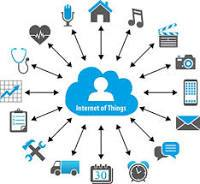
\includegraphics[width = 170 pt]{img.jpg}
\end{document}